\chapter{Configuring Networks with NETCONF}

In this chapter, we explore the practical implementation of NETCONF (Network Configuration Protocol) for configuring networks in a Cisco router. Building upon the foundational understanding of DHCP, NAT, SSH, and the fundamentals of NETCONF established earlier, we delve into the specifics of leveraging NETCONF to streamline network configuration processes.

Before delving further, it is crucial to first explore the fundamental base operations of NETCONF. Understanding these operations provides a solid foundation for effectively leveraging NETCONF in network configuration management.

\section{NETCONF base operations}

The NETCONF protocol supports a set of low-level operations for retrieving and managing device configuration information. The operations are specified through XML elements, which are described in the following table. NETCONF also supports additional operations based on each device's capabilities:

\begin{itemize}
    \item \textless{get}\textgreater{} : Retrieves all or part of the information about the running configuration and device state.
    \item \textless get-config\textgreater : Retrieves all or part of the configuration information available from a specified configuration datastore.
    \item \textless edit-config\textgreater : Submits all or part of a configuration to a target configuration datastore.
    \item \textless copy-config\textgreater : Creates or replaces a target configuration datastore with the information from another configuration datastore.
    \item \textless delete-config\textgreater : Deletes a target configuration datastore, but only if it's not running.
    \item \textless lock\textgreater : Locks a target configuration datastore, unless a lock already exists on any part of that datastore.
    \item \textless unlock\textgreater : Releases a lock on a configuration datastore that was previously locked through a \textless lock\textgreater operation.
    \item \textless close-session\textgreater : Requests the NETCONF server to gracefully terminate an open session.
    \item \textless kill-session\textgreater : Forces a session's termination, causing current operations to be aborted.
\end{itemize}

\section{Python Automation}

There are multiple ways to configure networks using NETCONF. Some common approaches include using command-line interfaces (CLI) on network devices, network management tools with built-in NETCONF support, or developing custom automation scripts. Python is a preferred choice for configuring networks with NETCONF due to its ease of use, rich ecosystem, comprehensive documentation, and most importantly, its integration capabilities.

\subsection{Python code structure}

\subsubsection{Libraries}

The ncclient library is a popular Python library used for interacting with NETCONF-enabled devices. It provides a high-level API (Application Programming Interface) that simplifies the process of establishing NETCONF sessions, retrieving device information, and configuring network devices. Its key benefits include:

\begin{enumerate}
    \item Simplified NETCONF Communication:
    \begin{itemize}
      \item Abstracts low-level details of the NETCONF protocol, providing an intuitive interface for developers.
      \item Allows developers to focus on automation logic without the need to delve into protocol intricacies.
    \end{itemize}
    
    \item Easy Connection Establishment:
    \begin{itemize}
      \item Handles authentication mechanisms (e.g., SSH) for establishing secure NETCONF sessions.
      \item Provides a seamless channel for communication with NETCONF-enabled devices.
    \end{itemize}
    
    \item Configuration Management:
    \begin{itemize}
      \item Facilitates retrieval and manipulation of device configuration using NETCONF.
      \item Simplifies the retrieval of configuration data, application of configuration changes, and validation of resulting configurations.
    \end{itemize}
    
    \item Error Handling and Validation:
    \begin{itemize}
      \item Includes built-in mechanisms for error handling and structured error responses.
      \item Enables developers to validate configuration changes and effectively handle exceptions.
    \end{itemize}

\end{enumerate}
\subsubsection{Session establishment}

In this section, we discuss the process of establishing a NETCONF session using the manager.connect() method as an example. This method is part of the ncclient library and allows us to establish a secure connection with the router.

\begin{figure}[h]
    \centering
    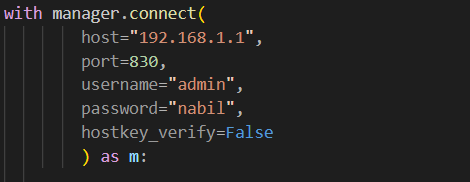
\includegraphics[width=0.5\linewidth]{Images/m_connect.png}
    \caption{Session establishment.}
\end{figure}

\begin{enumerate}
    \item \texttt{manager.connect()}: The \texttt{manager.connect()} method initiates the process of establishing a NETCONF session.
    \item \texttt{host}: This parameter specifies the IP address of the router (in this case, "192.168.1.1").
    \item \texttt{port}: The \texttt{port} parameter defines the port number used for the NETCONF communication, which is typically set to 830.
    \item \texttt{username} and \texttt{password}: These parameters provide the necessary authentication credentials to access the router.
    \item \texttt{hostkey\_verify}: By setting this parameter to \texttt{False}, host key verification for the SSH connection is disabled. This option can be useful during testing or when connecting to devices with self-signed or invalid SSH certificates. However, exercise caution and ensure the security implications are understood before using this option.
    \item \texttt{with} statement: The \texttt{with} statement ensures that the NETCONF session is properly established and automatically closed when the block of code inside the \texttt{with} statement finishes execution.
\end{enumerate}
\subsubsection{Filter}
The filter is a mechanism used to retrieve specific subsets of configuration or operational data from a network device. It allows us to define criteria for selecting the desired data elements using XPath expressions. By utilizing the filter parameter in NETCONF operations, such as <get-config> or <get>, we can retrieve only the relevant information needed for our application or task. This targeted data retrieval capability enhances network management and automation by minimizing unnecessary data transfer, optimizing response times, and reducing network bandwidth usage. 

For example, for the \texttt{<get-config>} operation in NETCONF with Python, we can use the \textit{filter} parameter to retrieve only the interface configurations from a network device. By specifying a filter criterion using XPath expressions that target the interface elements, such as \texttt{'/interfaces/interface'}, we can narrow down the retrieved data to only the relevant interface information.

\begin{figure}[h]
    \centering
    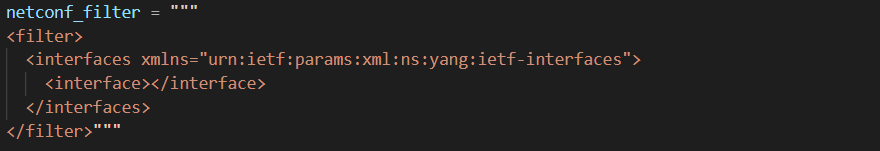
\includegraphics[width=0.8\linewidth]{Images/filter_int.png}
    \caption{Filter for interfaces.}
\end{figure}
\subsubsection{Base operation sending}